\documentclass[10pt,a4paper]{article}

%\usepackage{lipsum}
%\usepackage{here}
%\usepackage{qtree}
%\usepackage{amstext}
%\usepackage{multirow}
%\usepackage{subfigure}
%\usepackage{algorithm}
%\usepackage{algorithmic}
%\usepackage{listings}
%\usepackage{xcolor}

\usepackage{verbatim}
\usepackage{url}
\usepackage{amsmath}
\usepackage[UKenglish]{isodate}
\usepackage{graphicx}
\usepackage{multicol}
\usepackage{caption}
\usepackage{multicol}
\usepackage[margin=0.67in]{geometry} %margins usually 0.67

\begin{document}

\title{Automation of Crystal Orientation}
\author{Aidan  Boxall}
\maketitle

\begin{abstract}
Beamline I16 at Diamond light Source carries out experiments looking at subtle magnetic properties of crystals using x-ray diffraction. Due to the small
number of crystals handled at I16 compared to other beam lines they did not have an automated crystal orientation facility. The purpose of this project was
to produce python code that could provide an orientation matrix for a crystal of arbitrary orientation but known crystal structure.
\end{abstract}

\begin{multicols}{2}
\section*{Introduction}
The aim of this project was to produce a system for automating the orientation of crystsal samples in beamline I16 at Diamond Light Source. Crystal orienation has to be carried out at the start of every experiment. It is a time consuming and repetitive task which makes it well suited to automation. Crystal orientation has to be found by measuring Bragg reflections. It is not always possible to do it simply by eye as the samples can be in the order of tens of microns in size.

\subsection*{Method Steps}
There were a number of steps to be completed in order to orienate the crystal. Firstly the program had to determine the best Bragg reflections to measure. This was determined by a number of factors. Once the reflections have been chosen the code prints a Jython script to run the machine to collect the data. Once the data has been collected the nect step is to find the peaks in the data. Typically the data contains in the order of 10000 images and only around 3 or 4 peaks so this is an importatant step. Once the peaks have been found the image data has to be converted to vectors. This was one of the more challenging steps. A number of scripts had to be produced to calculte the vectors and extract the axis and angles required to rotate the vectors into the appropiate reference frame. Once the vectors were in the correct frame the next step was to match these vectors to the corrosponding vectors in the theoretical crystal Cartesian frame. Finally the orientation matrix U was found by finding the rotations which rotate the found vectors onto the the theorectical ones.

\section*{Choosing Bragg Reflections}
The first aim of the project was to write a python script that could choose appropriate Bragg reflections to use for crystal orientation. This was achieved 
by considering many factors and giving them appropriate weightings.
\subsubsection*{Rotational Symmetry}
The list of reflections to choose from was reduced by a filter which removes the Bragg reflections which have a higher order of rotational symmetry than the
 crystal. This was necessary because if the rotational symmetry of the Bragg reflections is higher than that of the crystal it is not possible to find 
 the correct orientation matrix all of the time. In this situation there will be a set of at least two possible non-equivalent orientation matrices and only
one will be the true orientation matrix of the crystal. 
\subsubsection*{Nearby Reflections}
It is important to consider how many reflections are nearby to the group under consideration. If the crystal has other reflection which occur at nearby
 values of two theta then it is possible they will appear on the detector whilst scanning for the desired reflections. This could be problematic if one
 reflections is so close to another that either they cannot be distinguished or they could be mistaken for one another.
\subsubsection*{Ideal Reflection Angle}
Ideally the two theta angle needs to be around 45 degrees. If the angle is too low shadowing can become a problem %CHECK was that right?
and if its too large then chi step would need to be very small. %CHECK was that right?
This would mean that the chi scans would be more time consuming to run.
\subsubsection*{Number of Reflections}
After applying the filter to remove groups of equivalent reflections that have a higher rotational symmetry than the crystal it is desirable to have as many 
reflections as possible in the chosen equivalent reflection group. The more reflections possible there are the more they are likely to  be picked up by the detector. Therefore making more data available to use to find an accurate orientation matrix.
\subsubsection*{Intensity}
Obviously reflections with a higher intensity are more desirable choices are they are easier to detect. 

\section*{Finding the Peaks}
Once the reflections had been scanned it was necessary to find the reflection peaks within the data. This was done using the following method. Normally when a scan is carried out a region of interest (ROI) is defined. This is the region of the scan image where the peaks are expected. The pixel value sums of the ROI for each are stored in a data file for the scan. If the ROI was not defined or defined incorrectly at the time the scan was taken the code produced allows for this by containing methods to define a ROI and find the pixel sums from the image data directly. This is not desirable though as it is time consuming to run. Once the ROI sums have been found the average and standard deviation of these values are calculated. This allows a minimum value for a ROI of a particular image to be considered high enough to contain a peak to be calculated. This is initially considered to be the mean value plus five standard deviations. The required number of standard deviations is reduced until a desired number of peaks are found or the number of standard deviations reaches two. It was decided pixel counts below the mean plus two standard deviations are not significant enough to be considered peaks.

To ensure that areas around the top of peaks were not counted as peaks the following method was used. The code searches for the ROIs with the highest pixel counts. Then it looks at the neighbouring images in the kphi and chi directions. It continues to look at neighbouring images until it finds images that have ROI counts below the current minimum. It then removes all the images within this rectangular area in chi-kphi space from mask array. The mask array is an array the same size and shape as the ROI sums array but simply records which images have already been used and should no longer be counted as peaks. After all the brightest ROIs have either been listed as having peaks or have been masked the next brightest set of ROIs is considered. This process is repeated unit there are no longer any points left unmasked above the minimum peak height or the desired number of peaks is found. Then as mentioned above if the desired number of peaks has not been found the minimum peak height is reduced and the entire process is repeated.  

Once a list of images containing peaks had been found the coordinates of the peaks within the images was found by assuming the peaks were the brightest pixel in the ROI.

\section*{Converting the Images to Vectors}
The first step to converting the images to vectors was to find the beam vectors in the lab frame. The vector requied is the momentum transfer vector 
\begin{center}
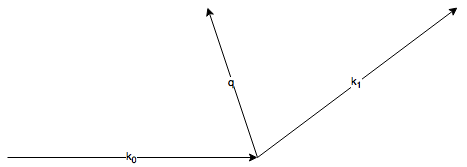
\includegraphics [width=\columnwidth]{vectors.png}
\captionof{figure}{Shows the relationship between the beam vectors and the momentum transfer vector: $\vec{q} = \vec{k_1}-\vec{k_0}$.}
\label{vectors}
\end{center}


\section*{Finding the Orientation Matrix}
Finding the orientation matrix was the most challenging and arguably the most important part of the project. Early in the planning it was realised an orientation matrix could be calculated by comparing two found momentum transfer vectors in the lab Cartesian frame to two theoretical momentum transfer vectors in the crystal Cartesian frame and finding the rotations required to transform one set to the other. The set of theoretical momentum transfer vectors consists of the entire set of vectors in the crystal's reciprocal space %CHECK is it actually all of them? Isn't reciprocal space infinite? Is it a unit cell of reciprocal space?
whereas the found vectors will be typically two to four vectors in lab Cartesian space. 
\subsection*{Finding the Matching Vectors in the Crystal Cartesian Frame}
To find the rotation that transforms one to the other it is required to find which vectors in the crystal frame correspond to the vectors in the lab frame. This requires a number of comparisons to ensure a valid set of vectors is chosen. Firstly the vectors moduli are compared to ensure they match. The vectors moduli physically corresponds to the two theta angle so must be the same for the same reflection. The angle between the vectors must also match. The angle between the vectors can be found by taking the dot product. By examining the moduli and the angle between the first pair of found vectors it is possible to find a matching pair in crystal Cartesian space. However, this is not necessarily sufficient to be sure that the correct pair has been found. This is only sufficient if the pair of vectors lie on a plane of symmetry in crystal Cartesian space. Otherwise there is an asymmetry about the chosen pair of vectors and without more information it is impossible to tell which way around the crystal is orientated. %This really needs a figure to illustrate this.
For example lets consider the case of a crystal containing three equivalent non-coplanar vectors as shown in Figure \ref{vectors1}
\begin{center}
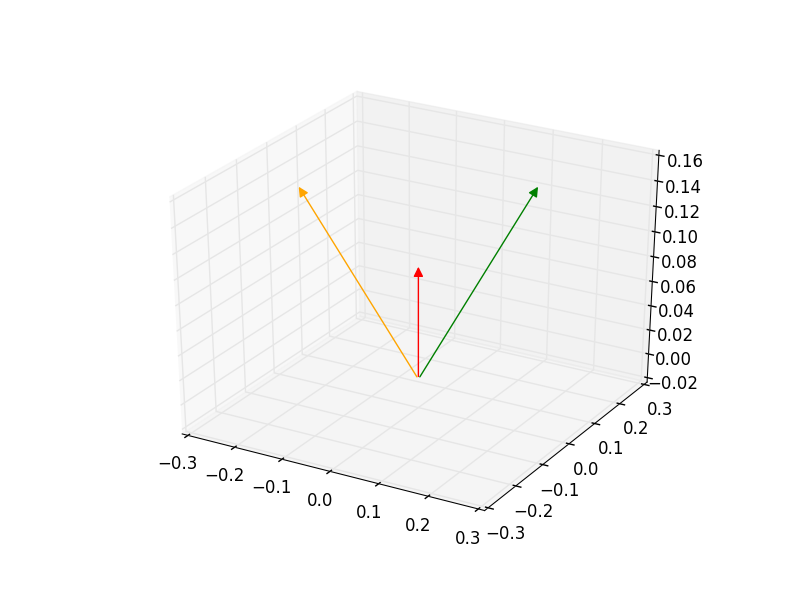
\includegraphics [width=\columnwidth]{three_vectors.png}
\captionof{figure}{Three equivalent non-coplanar vectors in the crystal Cartesian frame.}
\label{vectors1}
\end{center}
To provide an example it is assumed two vectors are found which match the red and green vectors in modulus and angle between them. Without further data it is not possible to tell which of the found vectors is the red or the green. This matters as without knowing which way round the red and green vectors there is no way to be certain where the orange vector is relative to the red and green vectors. It may be in the position of the orange vector or the crystal may be orientated such that it is in the position of the blue vector shown in Figure \ref{vectors2}. To find which way the crystal is in fact orientated a third vector needs to be considered.
\begin{center}
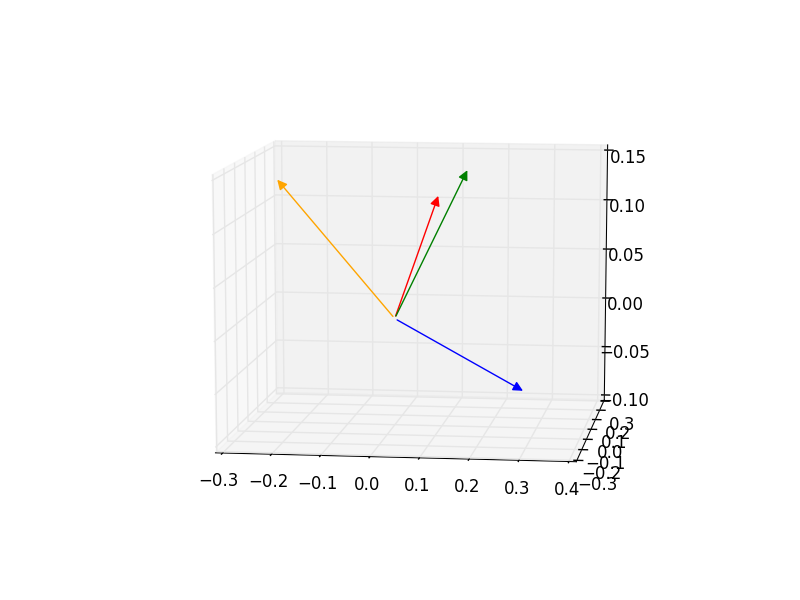
\includegraphics [width=\columnwidth]{four_vectors.png}
\captionof{figure}{This shows that if two vectors are found but it is not known which is which this leaves the position of the third vector ambiguous.}
\label{vectors2}
\end{center}
Let the vectors in the crystal Cartesian frame be labelled as follows: the red vector $\vec{r}$, the green vector $\vec{g}$ and the orange vector $\vec{o}$. Let the found vectors be labelled as follows: the red vector $\vec{r'}$, the green vector $\vec{g'}$ and orange vector $\vec{o'}$. In this example the blue vector doesn't correspond to anything physical but is just there for illustrate purposes. Assuming the red, green and orange vectors have been found a method to distinguish this from the red, green and blue vector set is required. This can be done by comparing $(\vec{r} \times \vec{g})\cdot \vec{o}$ to  $(\vec{r'} \times \vec{g'})\cdot \vec{o'}$. If $\hat{r'}=\hat{r}$, $\hat{g'}=\hat{g}$ and $\hat{o}=\hat{o'}$ then  $(\vec{r} \times \vec{g})\cdot \vec{o}$ should be the same sign as $(\vec{r'} \times \vec{g'})\cdot \vec{o'}$. If not this implies that the red and green vectors have been labelled the wrong way round.

If the third vector is not coplanar with the first then it is not possible to find which side of the first two it lies on by taking the dot product of the third vector with the cross product of the first two. This is because if they are coplanar the cross product will be a zero vector. If the three vectors are coplanar it is possible to match the third vector by the angles between them and moduli alone as shown in Figure \ref{coplanar}. 
\begin{center}
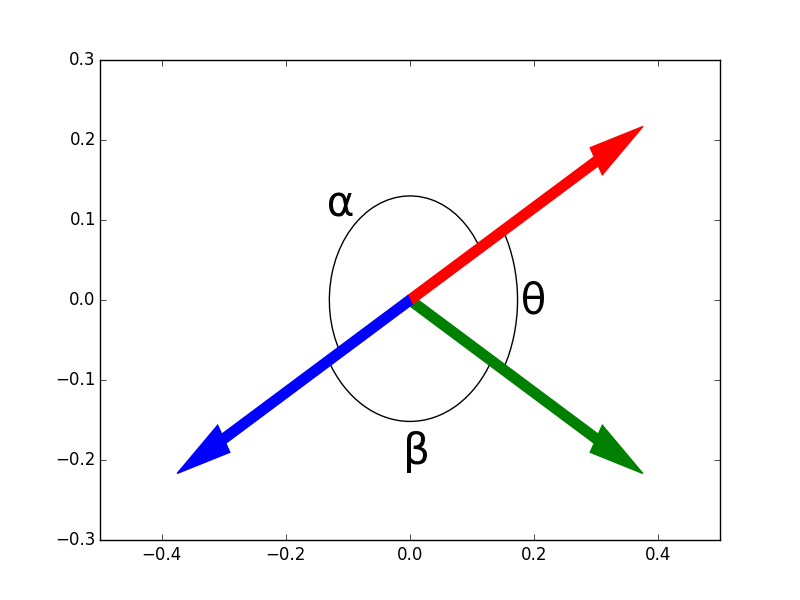
\includegraphics [width=5 cm]{angles.png}
\captionof{figure}{Finding a third coplanar vector using angles alone}
\label{coplanar}
\end{center}
This works in all cases except when the first two vectors are anti-parallel. If there first two vectors are anti-parallel then they are assumed to be on an plane of symmetry in reciprocal space. This is because if there is no asymmetry then either orientation is equivalent as shown in Figure \ref{anti-parallel}. In Figure \ref{anti-parallel} it is assumed the red and green vectors are the vectors which have been found. The choice of which way round red and green are labelled is arbitrary as the choice between the orange and blue vectors is arbitrary so either choice would produce a valid crystal orientation. Apart from coplanar vectors like this anti-parallel vectors cannot be used as the first two found vectors.
\begin{center}
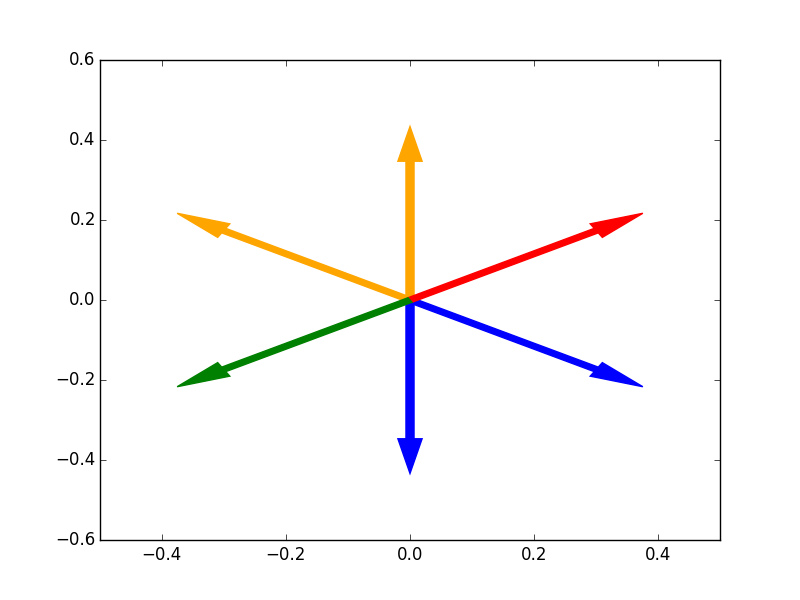
\includegraphics [width=5 cm]{coplanar.png}
\captionof{figure}{There is no asymmetry when the initial vectors are on a plane of symmetry. The choice of the orange or blue vectors is arbitrary.}
\label{anti-parallel}
\end{center}

\subsection*{Finding the Rotations}
Once the first two vectors have been matched to targets the rotations need to be found. The first rotation is used to rotate the first found vector onto the first target. It can be found by choosing an axis of rotation to be the cross product of the found and target vectors and the angle of rotation to be the angle between the vectors as shown in Figure \ref{rotation1}.
\begin{center}
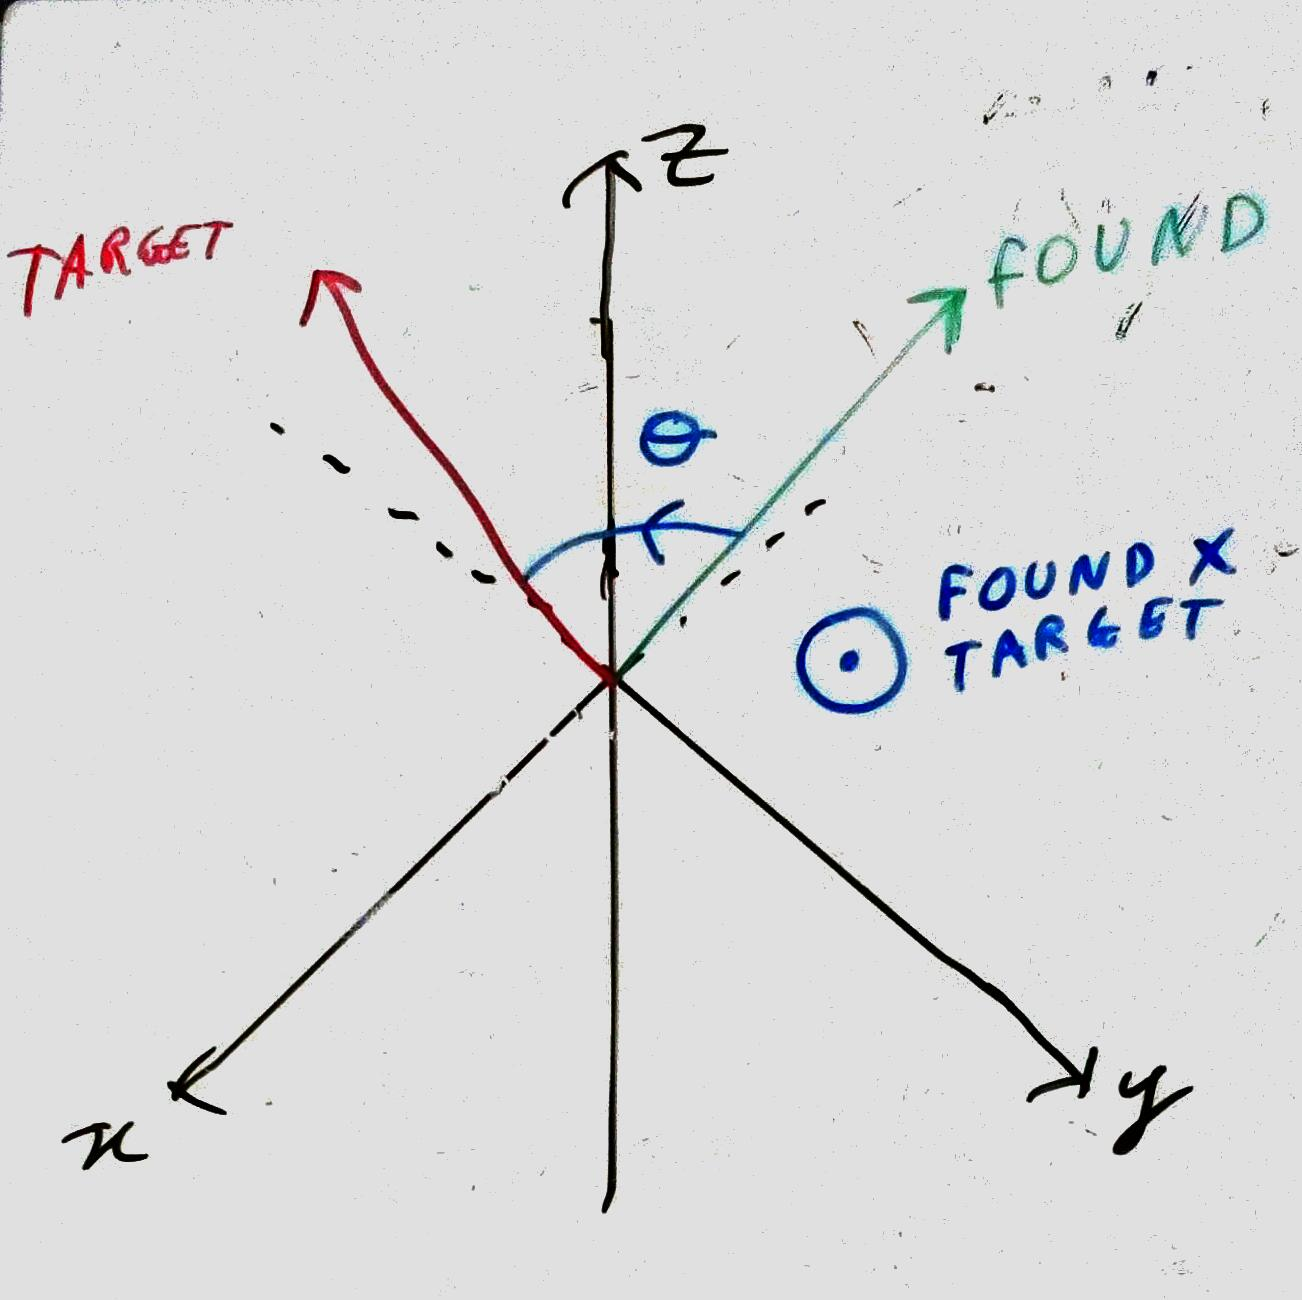
\includegraphics [width=5 cm]{rotation1.jpg}
\captionof{figure}{The first rotation.}
\label{rotation1}
\end{center}
This leaves the only possible rotation as one about the first target vector. The angle of this rotation is the angle between the components of the second found vector and the second target vector which are perpendicular to the first vector as shown in Figure \ref{rotation2}.
\begin{center}
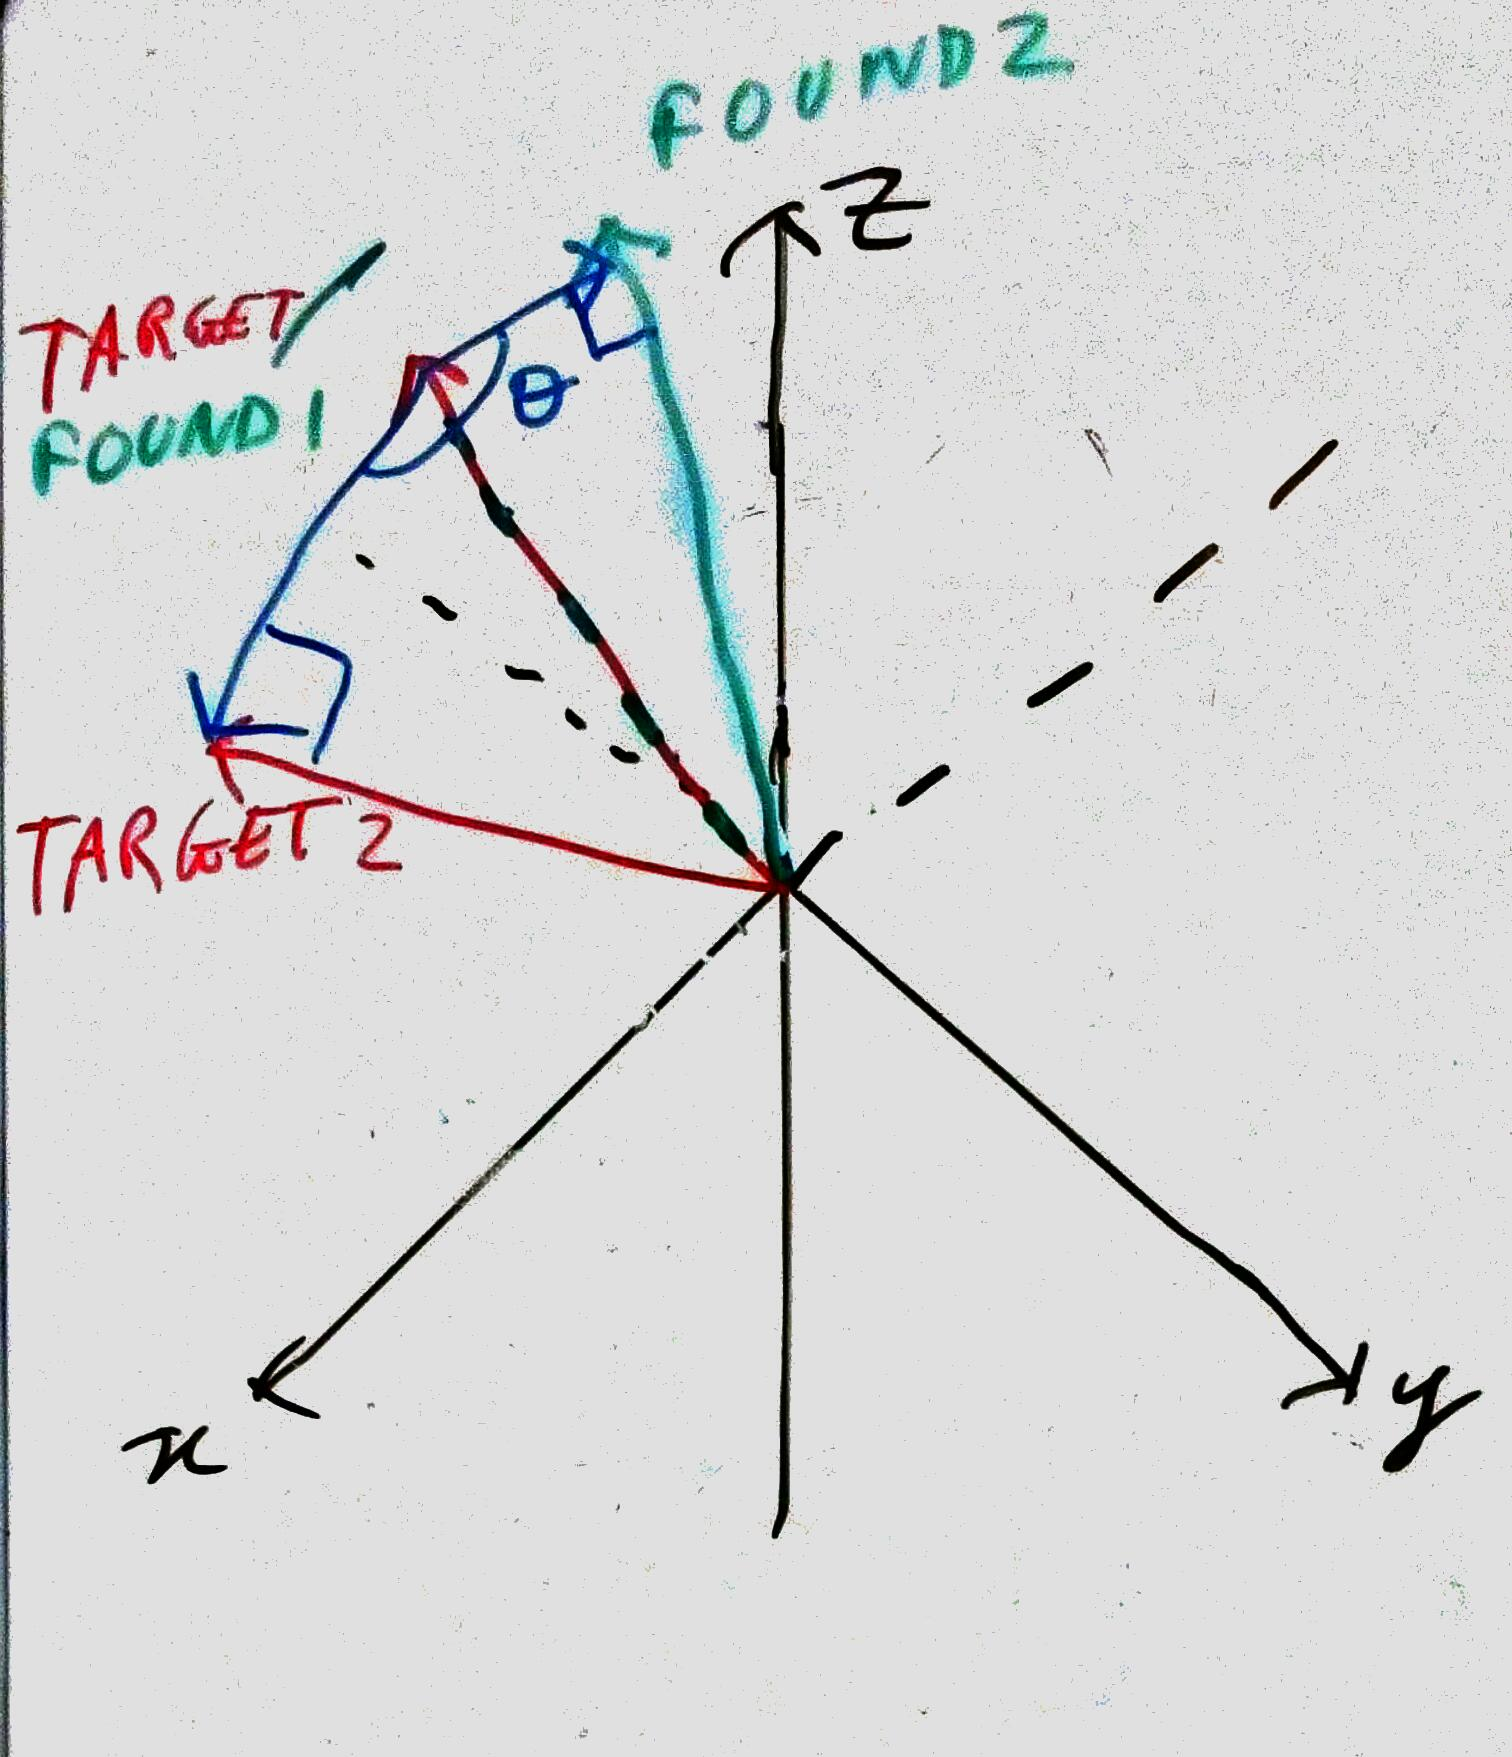
\includegraphics [width=5 cm]{rotation2.jpg}
\captionof{figure}{The second rotation.}
\label{rotation2}
\end{center}





\end{multicols}



\bibliographystyle{unsrt}
\bibliography{Bibliography}

\section*{Appendix}

\end{document}
